

\subsection{Iteración 2}

En esta iteración se busca crear en Unity las mecánicas básicas necesarias para realizar las distintas pruebas.


\subsubsection{Pruebas de posición} 
\label{E2_triggers}

Para implementar los triggers explicados en la iteración anterior se ha creado un objeto en Unity con forma de cubo y un tamaño que equivaldría a 50x50x50 centímetros en el mundo real. Durante el desarrollo del proyecto los triggers serán visibles para facilitar el trabajo, y serán de color rojo por defecto, pero se volverán verdes cuando detecten un mando en su interior, mostrando así su correcto funcionamiento.

Cada trigger contiene un único script que define su comportamiento durante el juego y es el encargado de detectar si hay un mando en su interior y reflejarlo de forma adecuada. El script utiliza las cinco variables mostradas en la figura \ref{fig:E2_variablesTriggers}, dos de ellas (‘correctMaterial’ e ‘incorrectMaterial’) son para almacenar los materiales que mostrará según haya o no algún mando en su interior. ‘controllerTag’ contiene el texto con el que se van a etiquetar los mandos, para de esta forma poder detectar si el objeto dentro del trigger es un mando. ‘nControllers’ almacena en todo momento el número de mandos que hay dentro del trigger, ya que es posible que haya varios en un mismo instante. Finalmente, ‘controllerInside’ contendrá un valor de verdadero o falso según haya algún mando en el trigger o no.


\begin{figure}
  \centering
    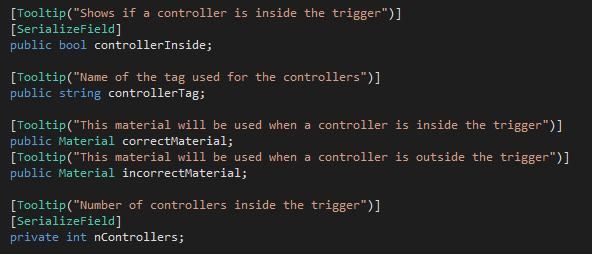
\includegraphics[width=0.9\textwidth]{04.Desarrollo/02.Entrega2/02.Iteracion2_2/00.Figuras/01.variables_trigger.png}
    \caption{Variables en el script para los triggers.}
    \label{fig:E2_variablesTriggers}
\end{figure}

Durante el juego este script detecta la entrada y salida de cualquier objeto en el trigger mediante dos funciones nativas de Unity: OnTriggerEnter y OnTriggerExit, como se muestra en la figura \ref{fig:E2_onTriggerEnter}. Las funciones se activan cuando se detecta un cualquier nuevo objeto, por lo que es necesario distinguir si se trata de un mando o no, para ello se utiliza la etiqueta “Controller” que está almacenada en la variable controllerTag. Si la etiqueta es la adecuada, quiere decir que un mando ha entrado o salido del trigger, por tanto, se actualiza el número de mandos que hay actualmente dentro del mismo.


\begin{figure}
  \centering
    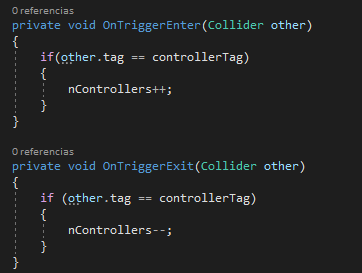
\includegraphics[width=0.7\textwidth]{04.Desarrollo/02.Entrega2/02.Iteracion2_2/00.Figuras/02.on_trigger_enter.png}
    \caption{Métodos para manejar la entrada y salida de objetos en un trigger.}
    \label{fig:E2_onTriggerEnter}
\end{figure}

Finalmente, el script comprobará de forma constante el número de mandos en su interior (figura \ref{fig:E2_updateTrigger}), en caso de no haber ninguno, pondrá la variable ‘controllerInside’ a falso y usará el material rojo, indicando que no hay mandos en su interior. En caso contrario, el trigger usará el material ‘correctMaterial’ para mostrar que hay al menos un mando en él, así como activar la variable ‘controllerInside’. Por último, como medida de seguridad se comprueba que el número de mandos dentro del trigger no sea menor que 0 ni mayor que 2, y en caso de darse dicha situación, reasigna el valor a 0 si era menor que 0 o a 2 si era mayor que 2.


\begin{figure}
  \centering
    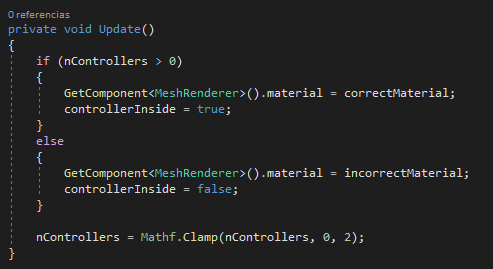
\includegraphics[width=0.7\textwidth]{04.Desarrollo/02.Entrega2/02.Iteracion2_2/00.Figuras/03.update_trigger.png}
    \caption{Parte del script que controla el número de mandos dentro de un trigger.}
    \label{fig:E2_updateTrigger}
\end{figure}

El siguiente problema planteado es la posición de los triggers en el espacio de juego.  Los triggers deben estar en una posición fija con relación al jugador, pero debido a la naturaleza de la realidad virtual, el jugador puede moverse y rotar libremente, lo que podría causar que los triggers no se encuentren en el lugar esperado por el jugador. Para solucionar este problema se ha diseñado una matriz de posiciones posibles en las que puede aparecer un trigger (mostrada en la figura \ref{fig:E2_spawnArray}), y esta matriz se encuentra ligada a la posición del jugador y se mueve junto a él. De este modo los triggers siempre aparecen en el mismo lugar con respecto al jugador.


\begin{figure}
  \centering
    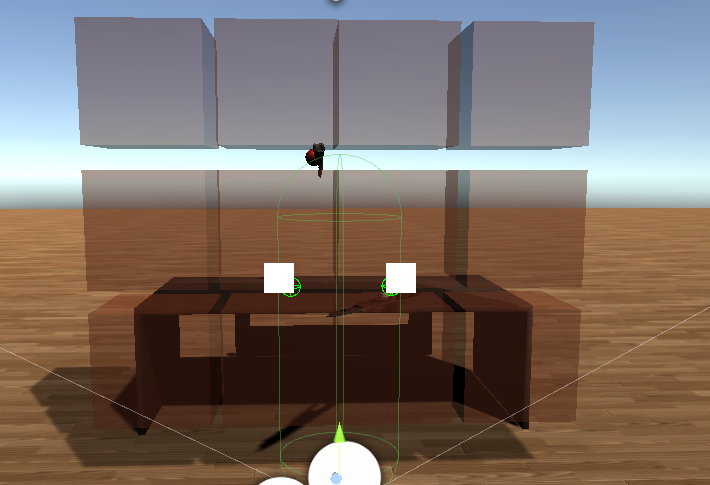
\includegraphics[width=0.7\textwidth]{04.Desarrollo/02.Entrega2/02.Iteracion2_2/00.Figuras/04.spawn_array.png}
    \caption{Representación de la matriz con 3 filas y 4 columnas de triggers. En el centro, una capsula verde representa al jugador, y los cubos blancos sus manos.}
    \label{fig:E2_spawnArray}
\end{figure}

A continuación, es necesaria una forma de crear los triggers necesarios para cada nivel en su posición correcta, así como un método para expresar la posición de cada trigger para cada nivel. Como primera solución a este problema se ha optado por diseñar usando JSON una forma de expresar las posiciones de la matriz que deben estar ocupadas por un trigger, usando un objeto en Unity capaz de leer dicho formato desde un fichero y cargar los triggers necesarios en el entorno virtual.

El formato elegido para la representación de un nivel en JSON se muestra en la figura \ref{fig:E2_json} y está compuesto por un campo “level” que encapsula todos los datos y contiene una lista de secciones llamada “part”. Cada sección corresponde a un estado concreto de la matriz de triggers, y cada uno de esos estados está definido por un “time” que indica cuantos segundos tardará en activarse dicho estado desde el comienzo de la prueba; y una matriz “triggerPositions” que contiene valores true/false dónde un ‘true’ significa que el trigger que ocupa dicha posición de la matriz estará activo y un false significa que no habrá ningún trigger en dicha posición.


\begin{figure}
  \centering
    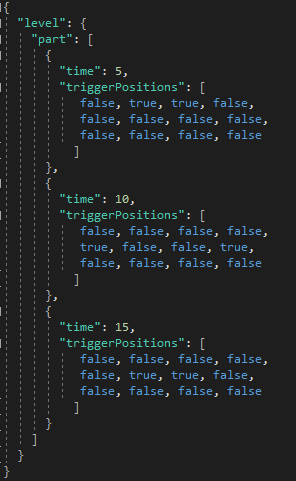
\includegraphics[width=0.4\textwidth]{04.Desarrollo/02.Entrega2/02.Iteracion2_2/00.Figuras/05.json.png}
    \caption{Ejemplo de la estructura JSON representando un nivel con 3 partes.}
    \label{fig:E2_json}
\end{figure}


En el ejemplo presentado en la figura 13 se muestra un nivel que empieza sin ningún trigger activo, a los 5 segundos del comienzo de la prueba se crean los dos triggers centrales de la primera fila. Pasados 10 segundos desde el comienzo, se desactivan los triggers anteriores y se activan los dos más exteriores de la fila central. Cinco segundos después se cargan los triggers finales, los centrales de la segunda fila.

Para las pruebas que requieren el movimiento de los mandos de un punto a otro, se puede crear un trigger aislado que siga una trayectoria a una velocidad determinada, pero teniendo este sistema de gestión de los triggers mediante una matriz y la capacidad de cargar mediante un fichero diferentes configuraciones de la misma que se modifiquen en momentos determinados, se puede modificar el procedimiento para las pruebas de movimiento de forma que se adapten a este sistema y faciliten el desarrollo del proyecto.

Con el primer diseño es necesario definir un punto de inicio del trigger (con los problemas respecto a su posición relativa explicados anteriormente), así como una serie de puntos intermedios junto con un tiempo que debe tardar el trigger en alcanzarlos. Usando el diseño desarrollado para los triggers estáticos se logra resolver tanto los problemas de posición relativa, mediante el uso de la matriz que sigue al jugador, como el problema del tiempo entre cada punto intermedio gracias a que se puede definir en el fichero el momento en el que aparecerá cada trigger. El único impedimento restante es contabilizar de manera correcta el movimiento del usuario de un trigger al siguiente con una velocidad adecuada. Para ello, el objeto controlador de la prueba se encarga de contar el tiempo que el jugador está fuera del trigger entre la primer y la segunda posición, de esta forma, se puede averiguar si el movimiento del jugador ha sido fluido y acorde a lo esperado. 

Esta solución para las pruebas de movimiento es menos precisa que la original, pero permite una mayor simplicidad y modularidad a la hora de construir niveles ya que se basa en el sistema desarrollado anteriormente.


\subsubsection{Pruebas de interacción}


Para este tipo de pruebas se diseñó en primer lugar utilizar los mismos triggers que se han usado hasta el momento, pero durante la implementación se ha encontrado una funcionalidad de VRTK que se ajusta más al resultado deseado: ‘InteractableSnapZone’. Estos son objetos que forman una zona en la que si se coloca un objeto, cuando se suelte dicho objeto este se moverá automáticamente para colocarse en una posición y orientación determinada (figura \ref{fig:E2_snapHighLights}) de forma que el objeto queda siempre colocado de la misma forma. Además, ofrece esta funcionalidad con un rango de acción variable, es decir, la distancia desde la cual será capaz de colocar un objeto en el lugar adecuado. 


\begin{figure}
  \centering
    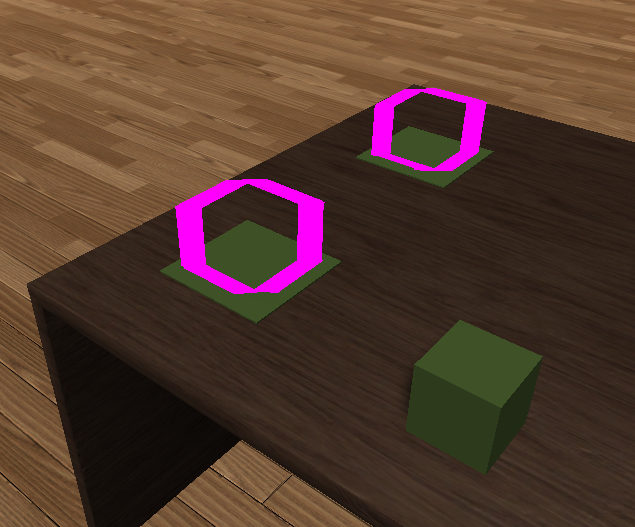
\includegraphics[width=0.5\textwidth]{04.Desarrollo/02.Entrega2/02.Iteracion2_2/00.Figuras/06.snap_highlights.png}
    \caption{Ejemplo que muestra dos plataformas verdes con dos InteractableSnapZone. En rosa se remarca la posición que ocupará el cubo verde si se suelta dentro de una de dichas zonas.}
    \label{fig:E2_snapHighLights}
\end{figure}

En la prueba de agrupación de objectos, que consiste en que al jugador se le presentan una serie de objetos y tiene que clasificarlos en dos grupos moviéndolos y colocándolos en sus zonas correspondientes, se usan dos zonas de snap y mediante un script se puede comprobar qué objetos hay en cada zona.


\begin{figure}
  \centering
    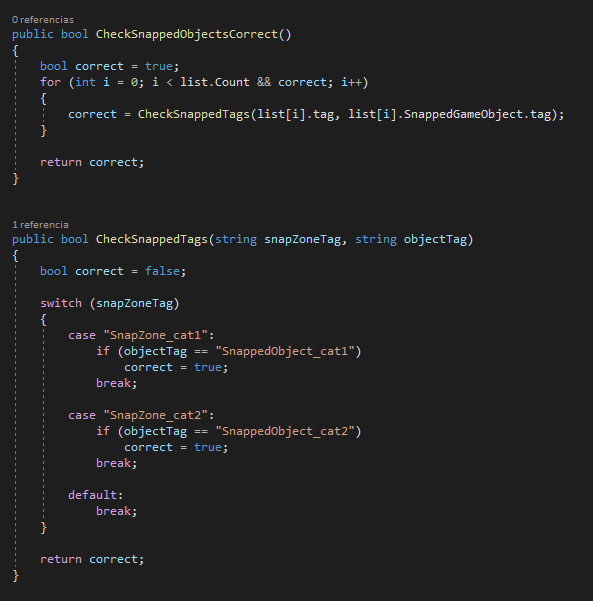
\includegraphics[width=0.8\textwidth]{04.Desarrollo/02.Entrega2/02.Iteracion2_2/00.Figuras/07.script_snap.png}
    \caption{Dos métodos del script que controla los objectos dentro de cada snap zone.}
    \label{fig:E2_scriptSnap}
\end{figure}

En el script presentado en la figura \ref{fig:E2_scriptSnap} aparecen dos de las funciones utilizadas para comprobar que cada snap zone contiene un objeto de la categoría que se desea. El método CheckSnappedObjectsCorrect recorre la lista ‘list’ que contiene todos los snap zones del nivel y para cada zona que hay en el nivel comprueba que tiene dentro un objeto de una categoría válida mediante la función CheckSnappedTags. Esta función compara la etiqueta que describe a la zona de snap con la etiqueta que describe al objeto de su interior, y en caso de ser de la misma categoría (en el ejemplo: cat1 o cat2), devuelve un valor verdadero que indica al controlador que el objeto es válido. Si existe alguna zona que contenga un objeto no válido, se da la prueba por fallida, pero en caso contrario la prueba habrá sido superada.

Para las pruebas de objetos superpuestos y de asociación de sonidos se utiliza un botón que el jugador tendrá que pulsar para indicar la respuesta correcta. La funcionalidad básica de los botones viene dada por SteamVR y consiste en un objeto que el jugador puede mover en un eje empujándolo con la mano (figura \ref{fig:E2_boton}). En este caso no es necesario agarrar el botón o interactuar de forma explícita con él, basta con que el jugador lo empuje para que el botón se active y ejecute un script, que es este caso indica si el botón pulsado es el correcto.


\begin{figure}
  \centering
    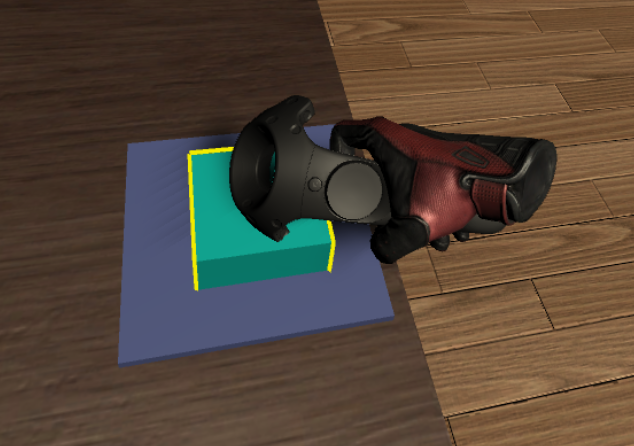
\includegraphics[width=0.5\textwidth]{04.Desarrollo/02.Entrega2/02.Iteracion2_2/00.Figuras/08.boton.png}
    \caption{Jugador pulsando un botón.}
    \label{fig:E2_boton}
\end{figure}

Finalmente, para la prueba de localización de sonidos se utiliza la capacidad que tiene Unity para generar audio 3D mediante el uso de su fuente de audio (figura \ref{fig:E2_audioSource}) junto con el espacializador de Oculus que es necesario configurar como se muestra en la figura \ref{fig:E2_audioSpatializer}. De esta forma solo en necesario colocar una fuente de sonido en cualquier punto alrededor del jugador y comprobar si está mirando hacia el origen del audio. Para hacer esta comprobación se usa una función del motor de renderizado de Unity que permite saber si un objeto va a ser dibujado en pantalla o no. Puesto que los objetos no visibles no se dibujan, de esta manera se determina si el jugador está viendo la fuente de audio mediante un sencillo script mostrado en la figura \ref{fig:E2_audioVisible}.

\begin{figure}
  \centering
    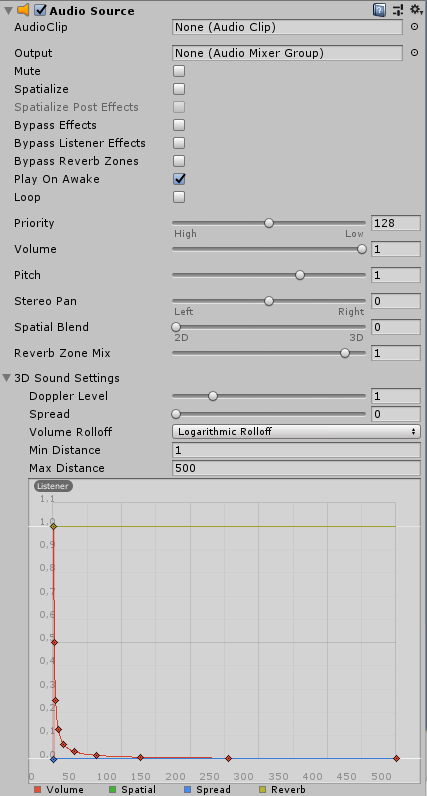
\includegraphics[width=0.5\textwidth]{04.Desarrollo/02.Entrega2/02.Iteracion2_2/00.Figuras/09.audio_source.png}
    \caption{Muestra de la configuración de una fuente de audio en Unity.}
    \label{fig:E2_audioSource}
\end{figure}

\begin{figure}
  \centering
    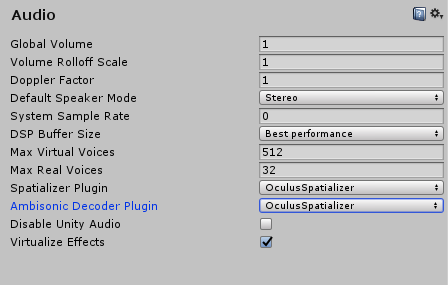
\includegraphics[width=0.5\textwidth]{04.Desarrollo/02.Entrega2/02.Iteracion2_2/00.Figuras/10.audio_spatializer.png}
    \caption{Ventana de configuración en la que es necesaria seleccionar OculusSpatializer para utilizar el sonido 3D.}
    \label{fig:E2_audioSpatializer}
\end{figure}

\begin{figure}
  \centering
    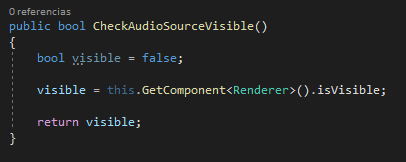
\includegraphics[width=0.5\textwidth]{04.Desarrollo/02.Entrega2/02.Iteracion2_2/00.Figuras/11.audio_visible_script.png}
    \caption{Método que comprueba si la fuente de audio es visible por el jugador. Este script debe estar en la propia fuente.}
    \label{fig:E2_audioVisible}
\end{figure}

Con esto quedan implementadas en el proyecto todas las mecánicas básicas que son necesarias para comprobar si el jugador realiza las pruebas de manera correcta o no.

